\chapter{Digital Filter FIR}
A digital filter is a system performing a certain function on an input stream $ X[n] $ (samples are received at constant rate) and generating an output stream called $ Y[n] $. 
In general it's possible to have multiple input streams and multiple output streams (for example in a parallel architecture this allows to speed up the filter).
\section{Digital filters properties}
Filters are systems characterized by the following properties:
\begin{enumerate}
	\item \textbf{Linearity}: it is possible to represent the output as an overlapping of the input pulses. Let $\delta[n-k]$ be the input signal and $ h_{k}[n] $ the filter response, using overlapping property, assuming that the input is a sum of pulses: 
	\begin{center}
		$ x[n]=\sum\limits_{k}^{} (x[n]\cdot \delta[n-k]) $
		\end{center}
		so the output is: $ h_{k}[n] =F(\delta[n-k])$ (F is the filter funtion), so applying linearity: 
			\begin{center}
				$ F(x[n])=F(\sum\limits_{k}^{ } (x[n]\cdot \delta[n-k])) $\\
			\end{center}
			\begin{center}
				$ y[n]=\sum\limits_{k}^{ } x[n]\cdot h_{k}[n] $
			\end{center}
    It means that if the input is a weighted sum of pulses, also the output will have the same form.
    \item  \textbf{Time invariance}: the shape of the answer $ h_{k} $ is not dependent on the selected time $ k $. So applying the same input signal at different time (i.e. different $ k $), the filter response will be always the same, just time-shifted. Therefore:
    
    \begin{center}
    	$ h_{k}[n] = h[n-k]  $
    \end{center}
    The expression for the output found before can be rewritten as:
    \begin{center}
    	$ y[n]=\sum\limits_{k}^{ } x[n]\cdot h_{k}[n]= \sum\limits_{k}^{ } x[n]\cdot h[n-k]=x[n]\ast h[n]$
    \end{center}
    where it has been used the definition of convolution product.
    \item \textbf{Stability}: we expect to have at the output a stable stream of samples whose values do not diverge. This is true if a sufficient numbers of bit has been employed for representing the samples. Assuming that the system is BIBO (bounded input bounded output), the following condition should be satisfied: 
    \begin{center}
    	$ S=\sum\limits_{k}^{ } |h[n]| < \infty $
    \end{center}
    \item \textbf{Causality}: if we apply an input at time $ k $,
     we expect that the output doesn't come before time $ k $.
     Assuming that $ x[n] = 0  $ for $ n < 0 $, then $ y[n] = 0 $ for $ k < 0 $: this property is true only if $  h[n] = 0 $ for $ n < 0 $
    
\end{enumerate}

\section{Hardware Implementation}
An FIR filter can be easily implemented using just three digital hardware elements, a unit delay (D Flip Flop), a multiplier, and an adder. The unit delay simply updates its output once per sample period, using the value of the input as its new output value. In the convolution sum,

\begin{center}
	$ 	 y[n]=\sum\limits_{k}^{ } x[n]\cdot h[n-k] =\sum\limits_{k}^{ } x[n-k]\cdot h[n]$
\end{center}
notice that at each $ n $ we need access to $ x(n)$, $x(n - 1)$, $x(n - 2)$, $\cdots$, $x(n - k) $. We can maintain this set of values by cascading a set of D Flip Flops to form a delay line, as shown in Fig. \ref{fig:fir1}
\begin{figure}[h!]
	\centering
	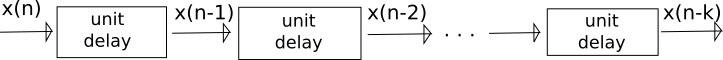
\includegraphics[width=0.9\textwidth]{imm/fir/fir1.png}  
	\caption{Cascading D Flip Flops} 
	\label{fig:fir1}
\end{figure}

For each of the previous $ k $ inputs, we have to scale them by $ h(0) $, $ h(1) $, $ \cdots $, $ h(k) $. To obtain these values, we simply put a multiplier as shown in the following picture (Fig. \ref{fig:fir2}).
To obtain the final result, we have to sum all the results of these multiplications.
\begin{figure}[h!]
	\centering
	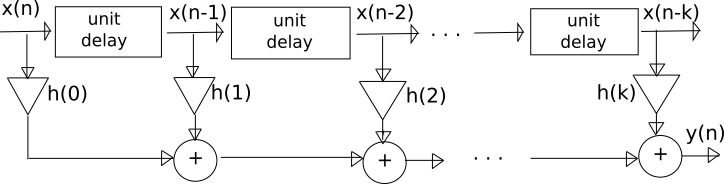
\includegraphics[width=0.9\textwidth]{imm/fir/fir2.png}  
	\caption{FIR hardware implementation} 
	\label{fig:fir2}
\end{figure}
\section{Simulation}
The simulation shown in this work has 6 constants (fig. \ref{fig:fir_sim}, \textit{fir\_constants\_value} section)
\begin{center}
	$ h_{0}=12$\\
	$h_{1}=10$\\
	$h_{2}= 8$\\
	$h_{3}= 6$\\
	$h_{4}= 4$\\
	$h_{5}= 2$\\
\end{center}
and it will take into account the last 6 inputs.\\
\begin{figure}[h!]
	\centering
	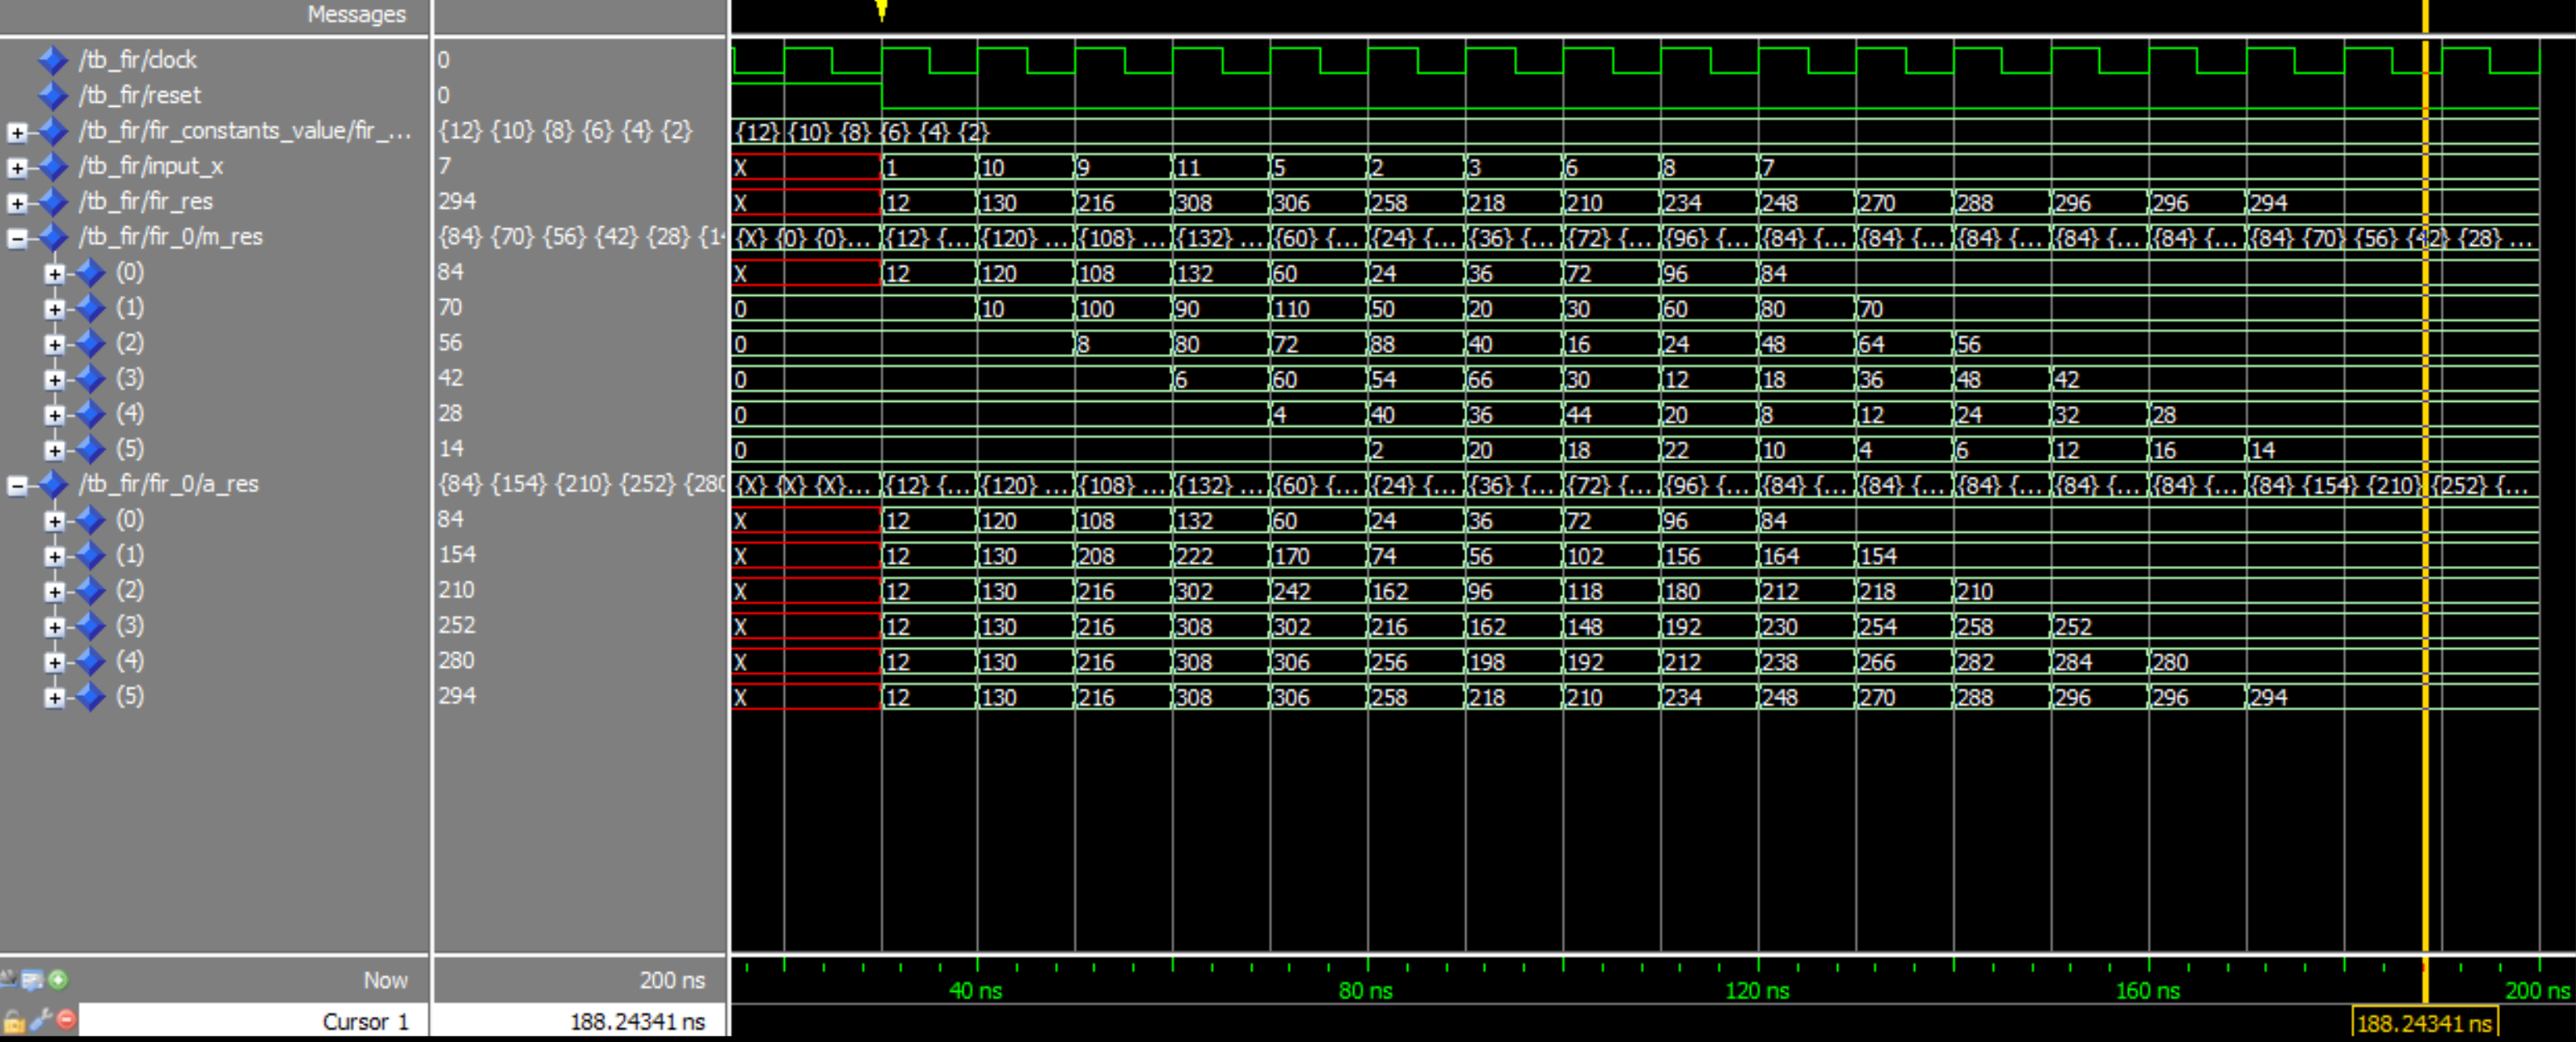
\includegraphics[width=\textwidth]{imm/fir/fir_sim.png}  
	\caption{FIR's simulation} 
	\label{fig:fir_sim}
\end{figure}
When we start sampling after the reset, we set all the previous inputs to $ '0' $, therefore the output will be simply $ y[n]=x[n]\cdot h_{0} $.\\
In fact in the simulation, as soon as the reset was set low, we see the output (fig. \ref{fig:fir_sim},\textit{fir\_res} signal) to be\begin{center}
	 $ y[n]=x[n]\cdot h_{0}=1\cdot12=12 $.
\end{center}
In the next cycle we get \begin{center}
	$ y[n]=x[n]\cdot h_{0}+x[n-1]\cdot h_{1}=10\cdot12+1\cdot 10=130 $.
\end{center}
For the next clock cycles we repeat the same procedure.\\
In the end, when the input has not changed for more than 6 clock cycles, we can see the result to be 
\begin{center}
	$ y[n]=\sum\limits_{k=0}^{6 } x[n-k]\cdot h[k]=7\sum\limits_{k=0}^{6 }=7\cdot42=294$
\end{center}

